\chapter{Invariant mass fits to $\Bd\to\Kstarz\ee$ simulated candidates}
\label{app:RKMCfits}

This appendix contains fits to the $m(K\pi ee )$ invariant mass of $\Bd\to\Kstarz\ee$ simulated candidates
used to constrain parameters in the fit to data.

\begin{figure}[h!]
\centering
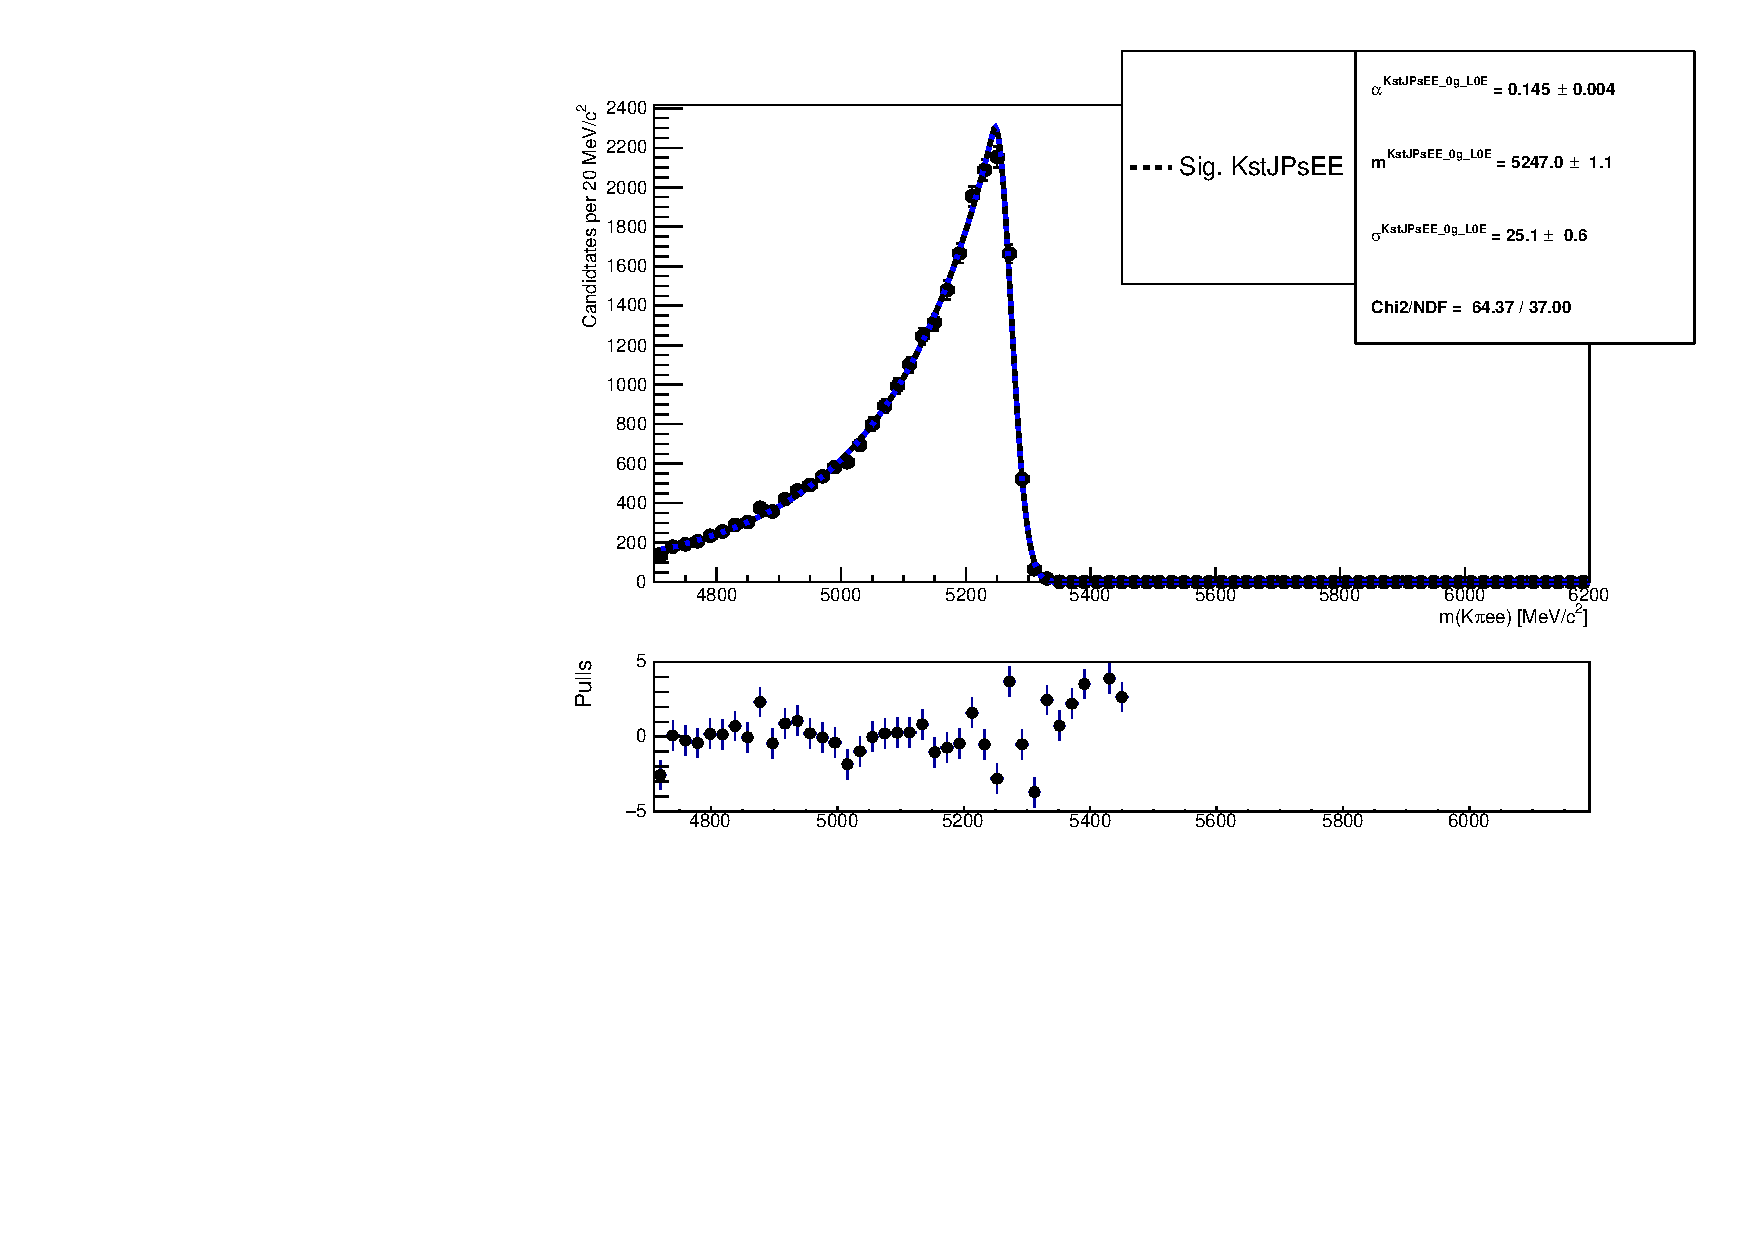
\includegraphics[width=0.6\textwidth]{RKst/figs/fit_EEs_0_EE-q2central-gmc/KstJPsEE_0g_L0E_fitAndRes.pdf}
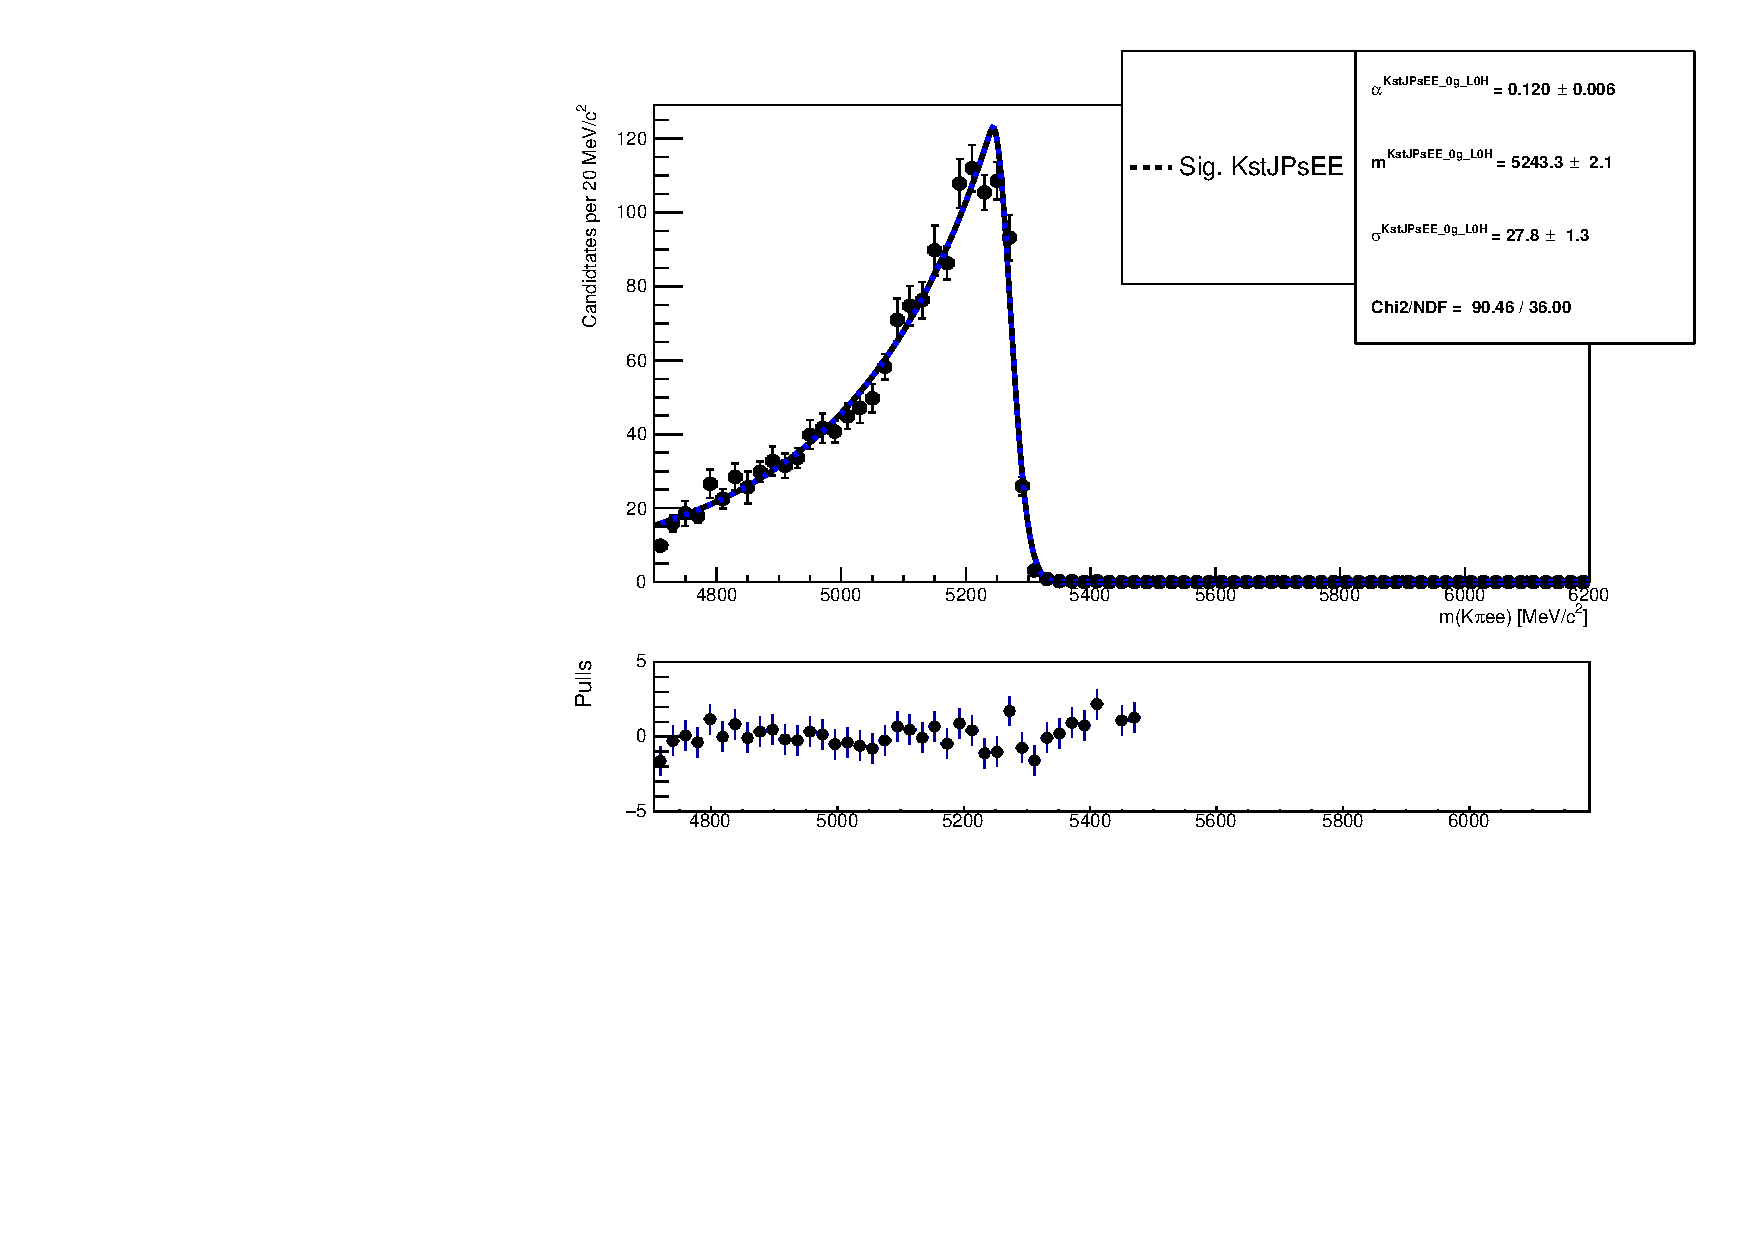
\includegraphics[width=0.6\textwidth]{RKst/figs/fit_EEs_0_EE-q2central-gmc/KstJPsEE_0g_L0H_fitAndRes.pdf}
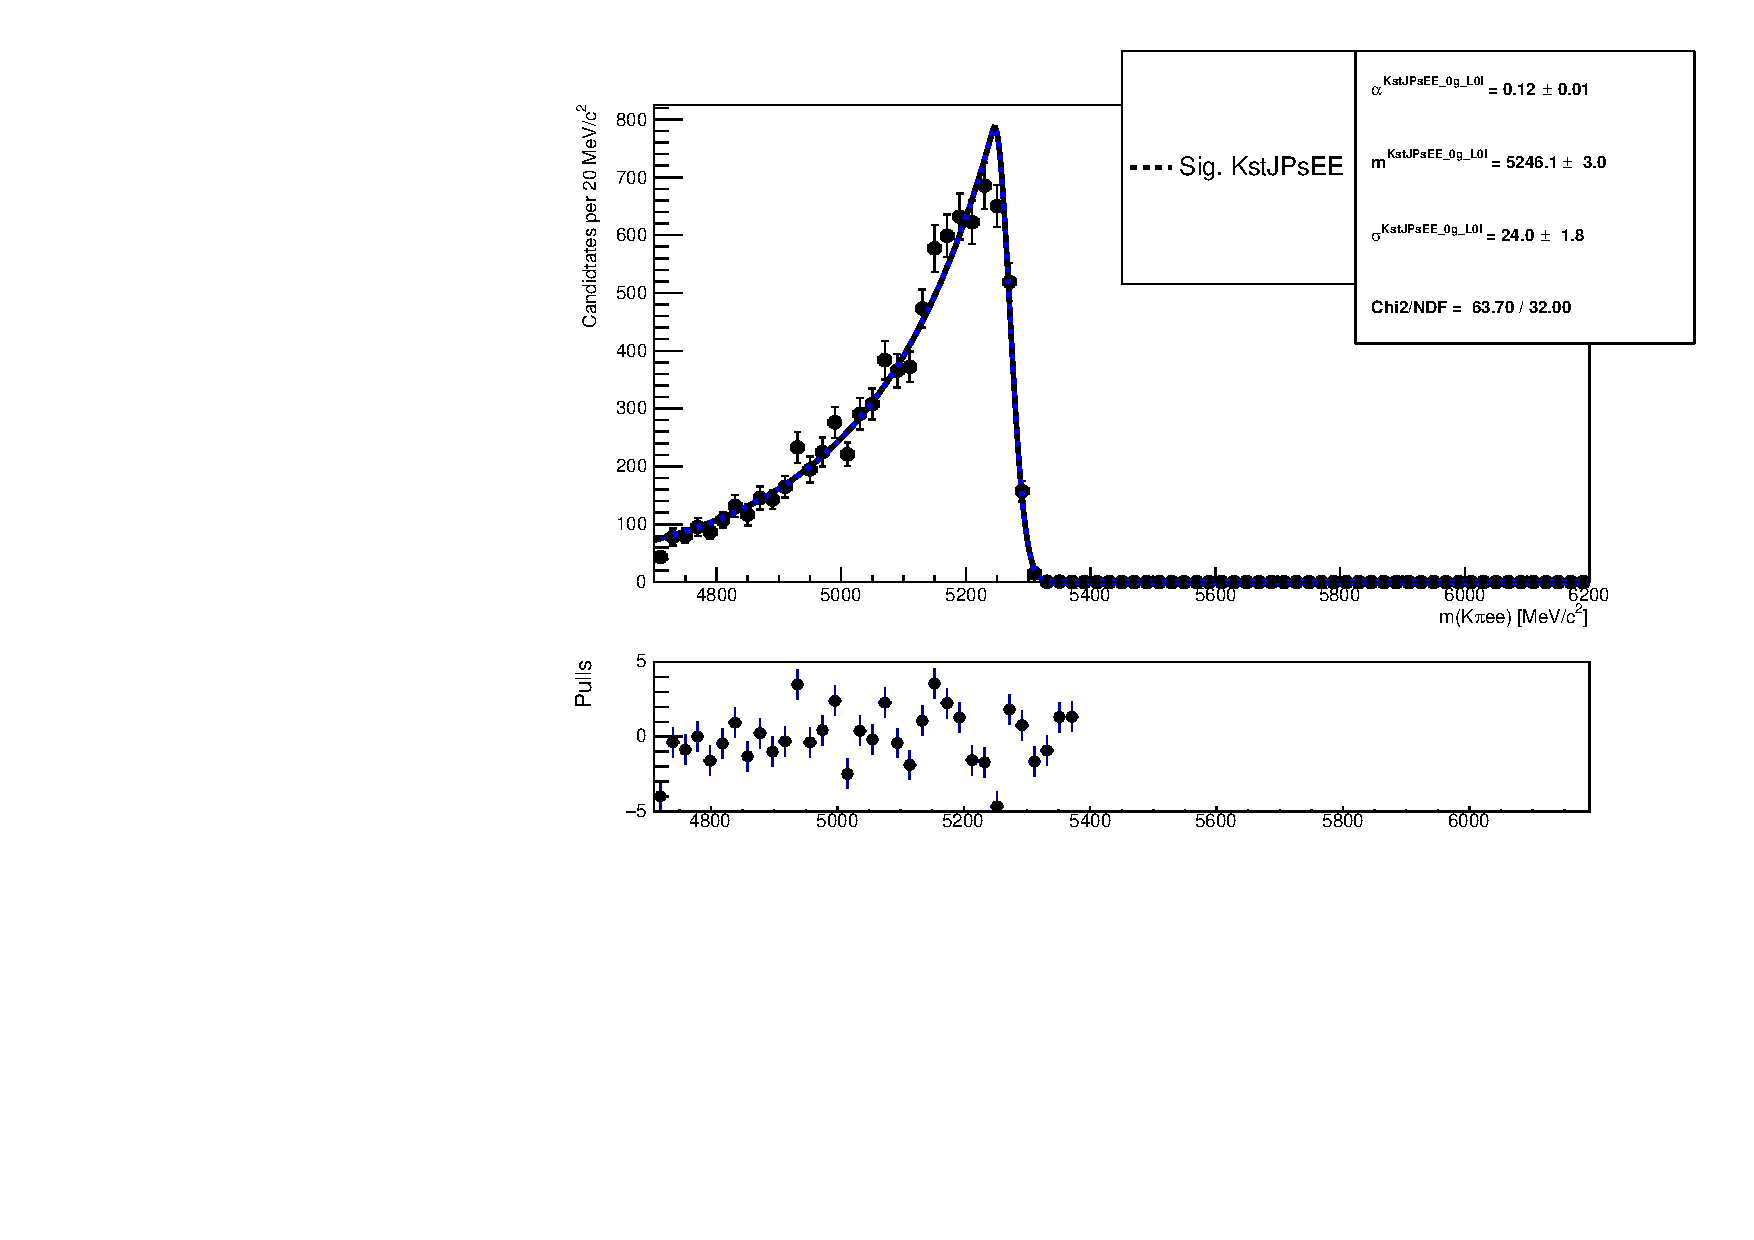
\includegraphics[width=0.6\textwidth]{RKst/figs/fit_EEs_0_EE-q2central-gmc/KstJPsEE_0g_L0I_fitAndRes.pdf}
\caption{Fitted $m(K\pi ee)$ mass spectrum of $B^0 \rightarrow K^{*0} J/\psi(J/\psi\rightarrow ee)$ simulated
events in the three trigger categories and no photon emitted. }
\label{fig:FitEE_MC_inTrigCat_Brem0}
\end{figure}
%
%\clearpage
\begin{figure}[h!]
\centering
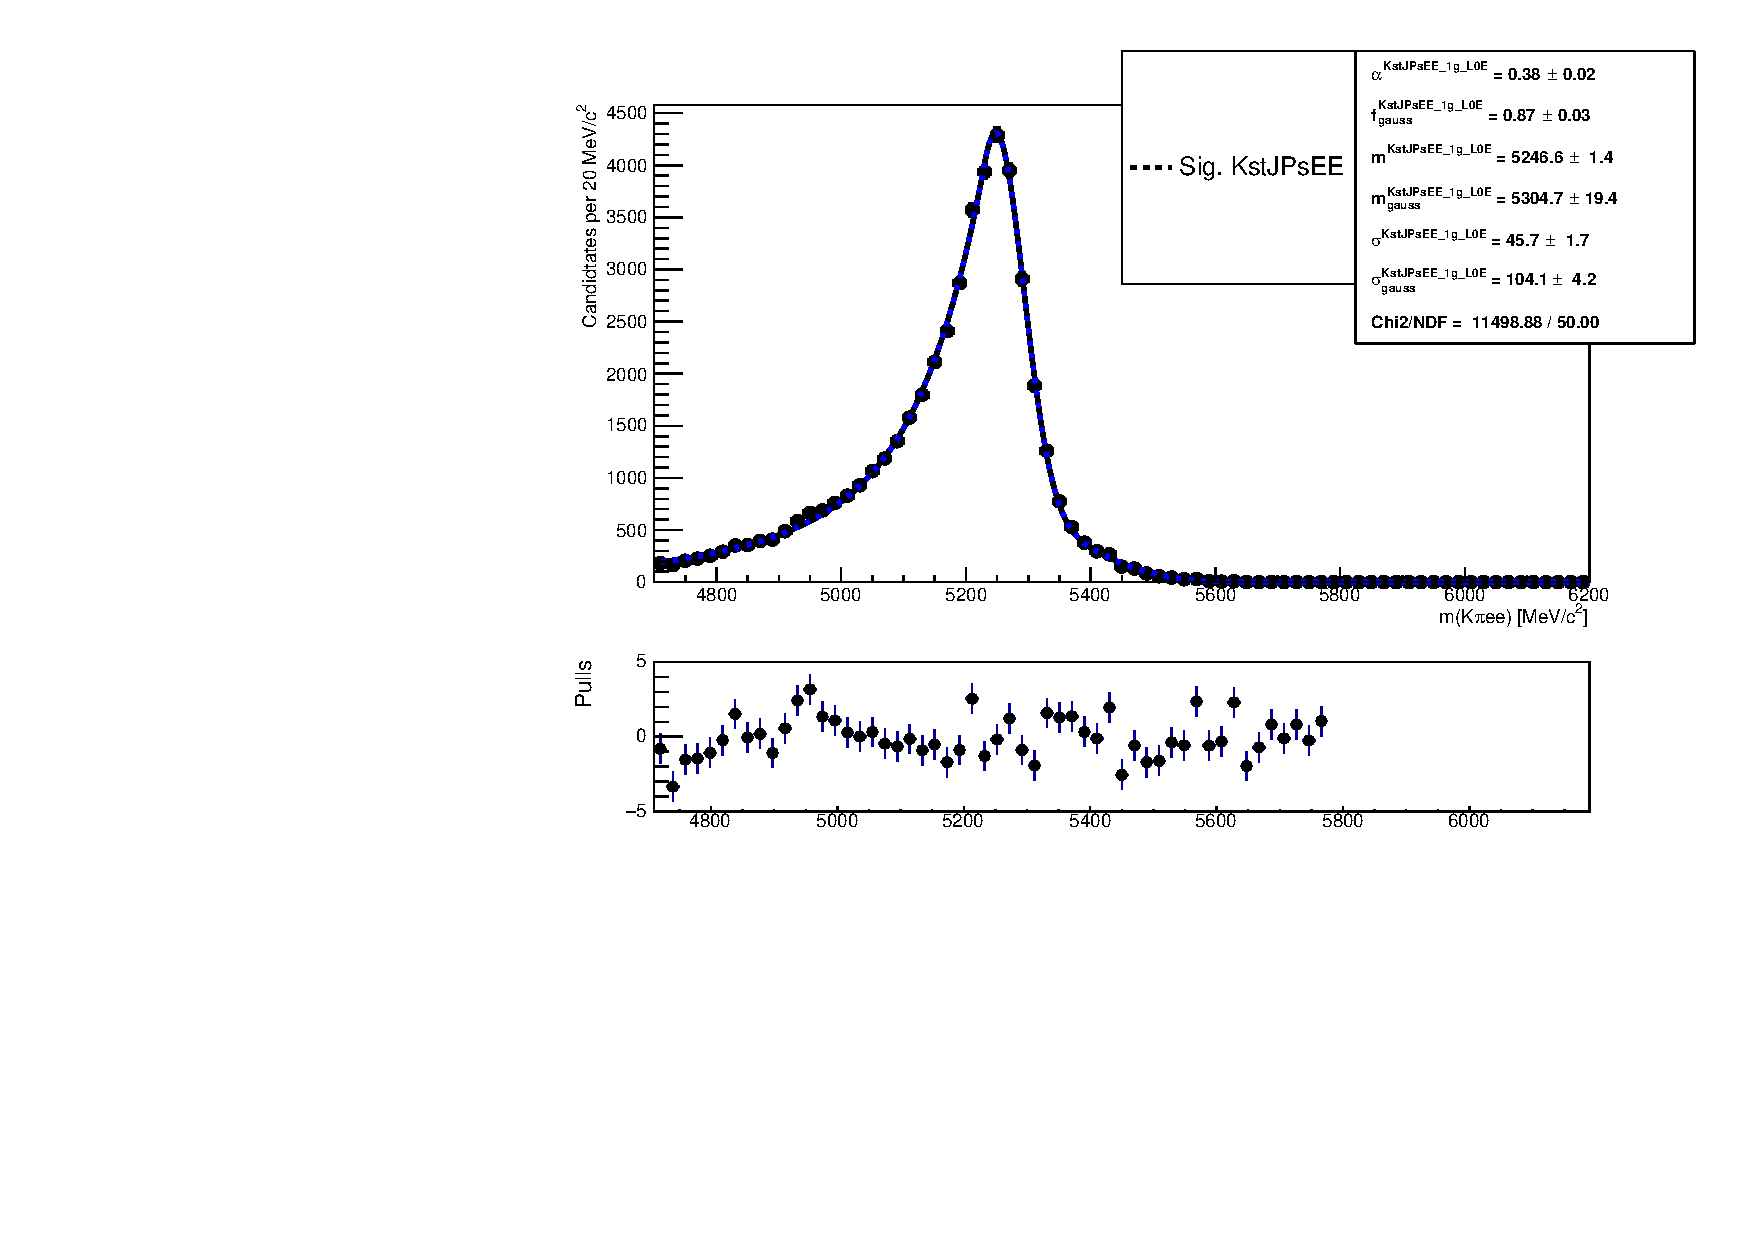
\includegraphics[width=0.6\textwidth]{RKst/figs/fit_EEs_0_EE-q2central-gmc/KstJPsEE_1g_L0E_fitAndRes.pdf}
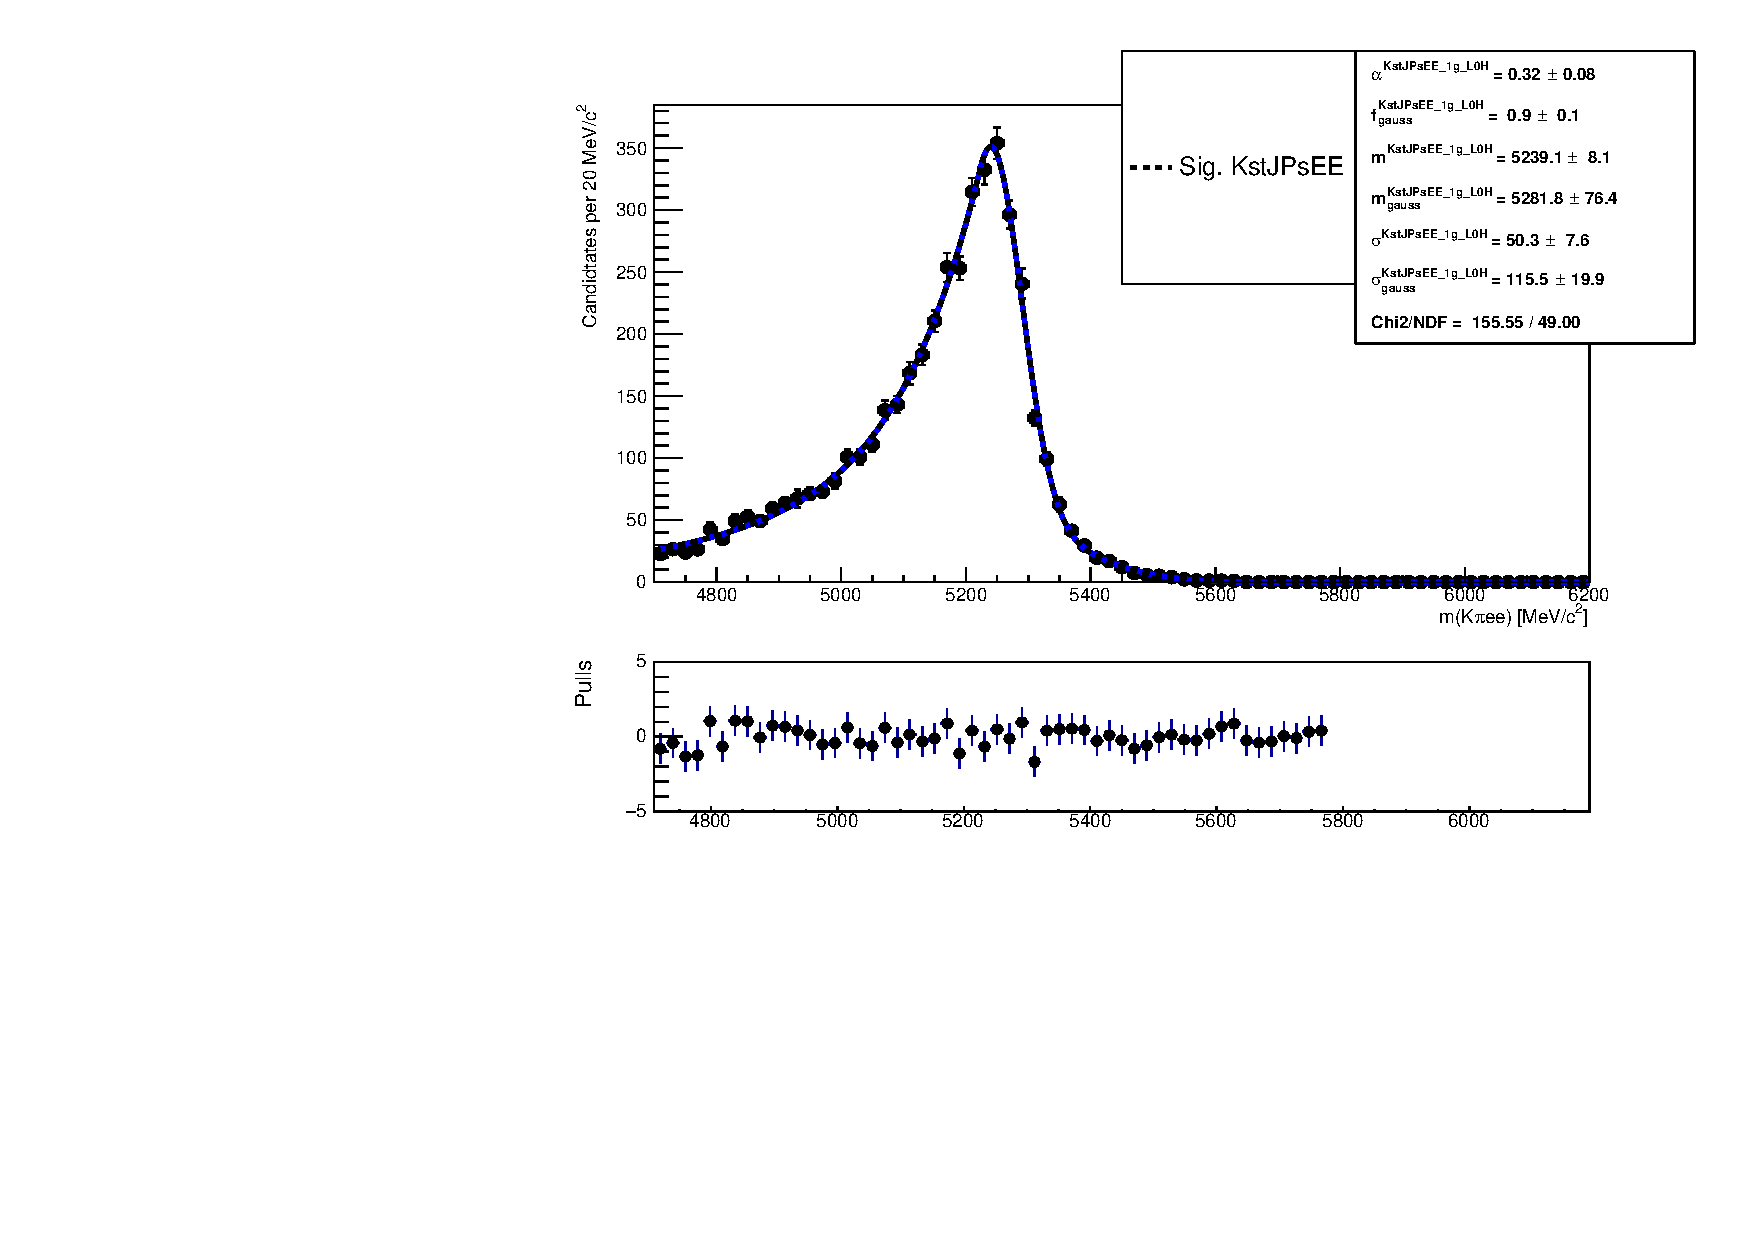
\includegraphics[width=0.6\textwidth]{RKst/figs/fit_EEs_0_EE-q2central-gmc/KstJPsEE_1g_L0H_fitAndRes.pdf}
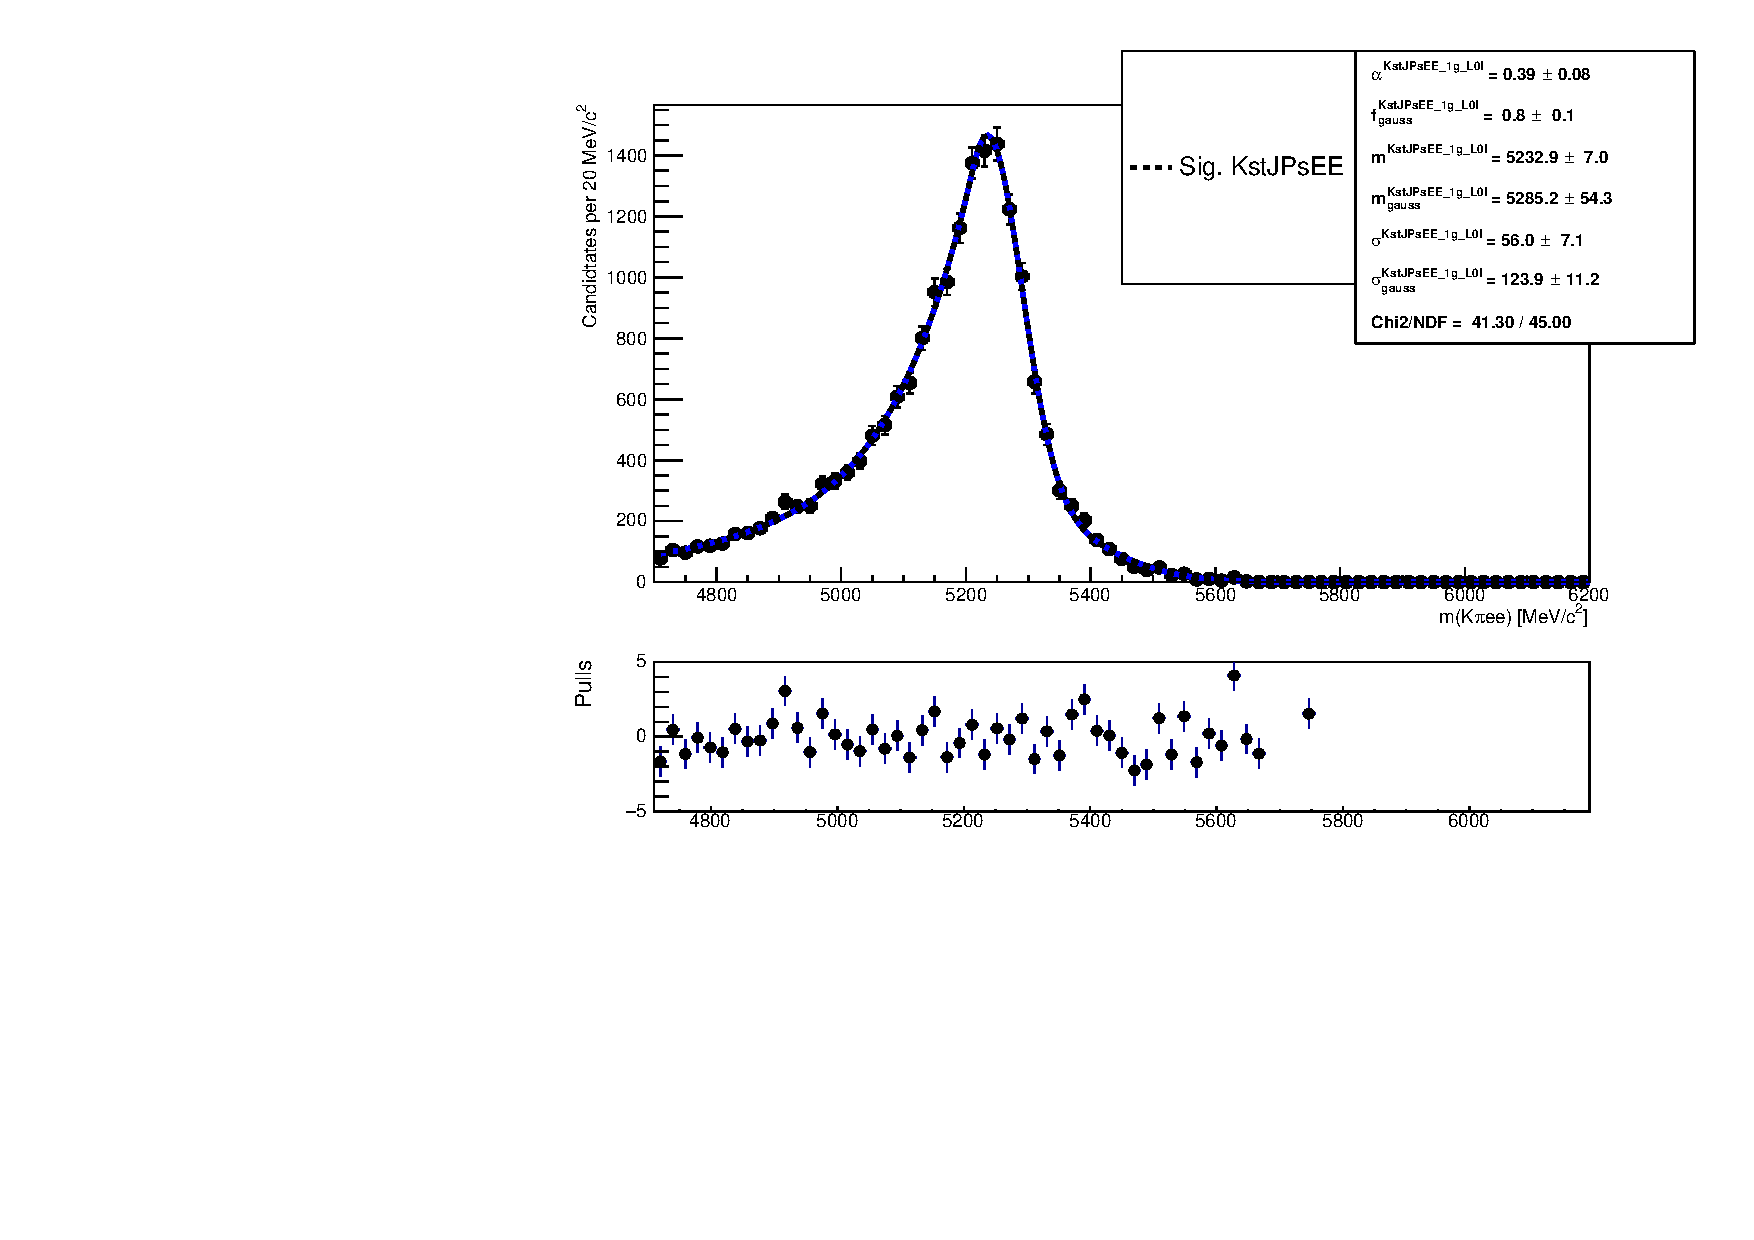
\includegraphics[width=0.6\textwidth]{RKst/figs/fit_EEs_0_EE-q2central-gmc/KstJPsEE_1g_L0I_fitAndRes.pdf}
\caption{Fitted $m(K\pi ee)$ mass spectrum of $B^0 \rightarrow K^{*0} J/\psi(J/\psi\rightarrow ee)$ simulated
events in the three trigger categories and one photon emitted. }
\label{fig:FitEE_MC_inTrigCat_Brem1}
\end{figure}
%
\begin{figure}[h!]
\centering
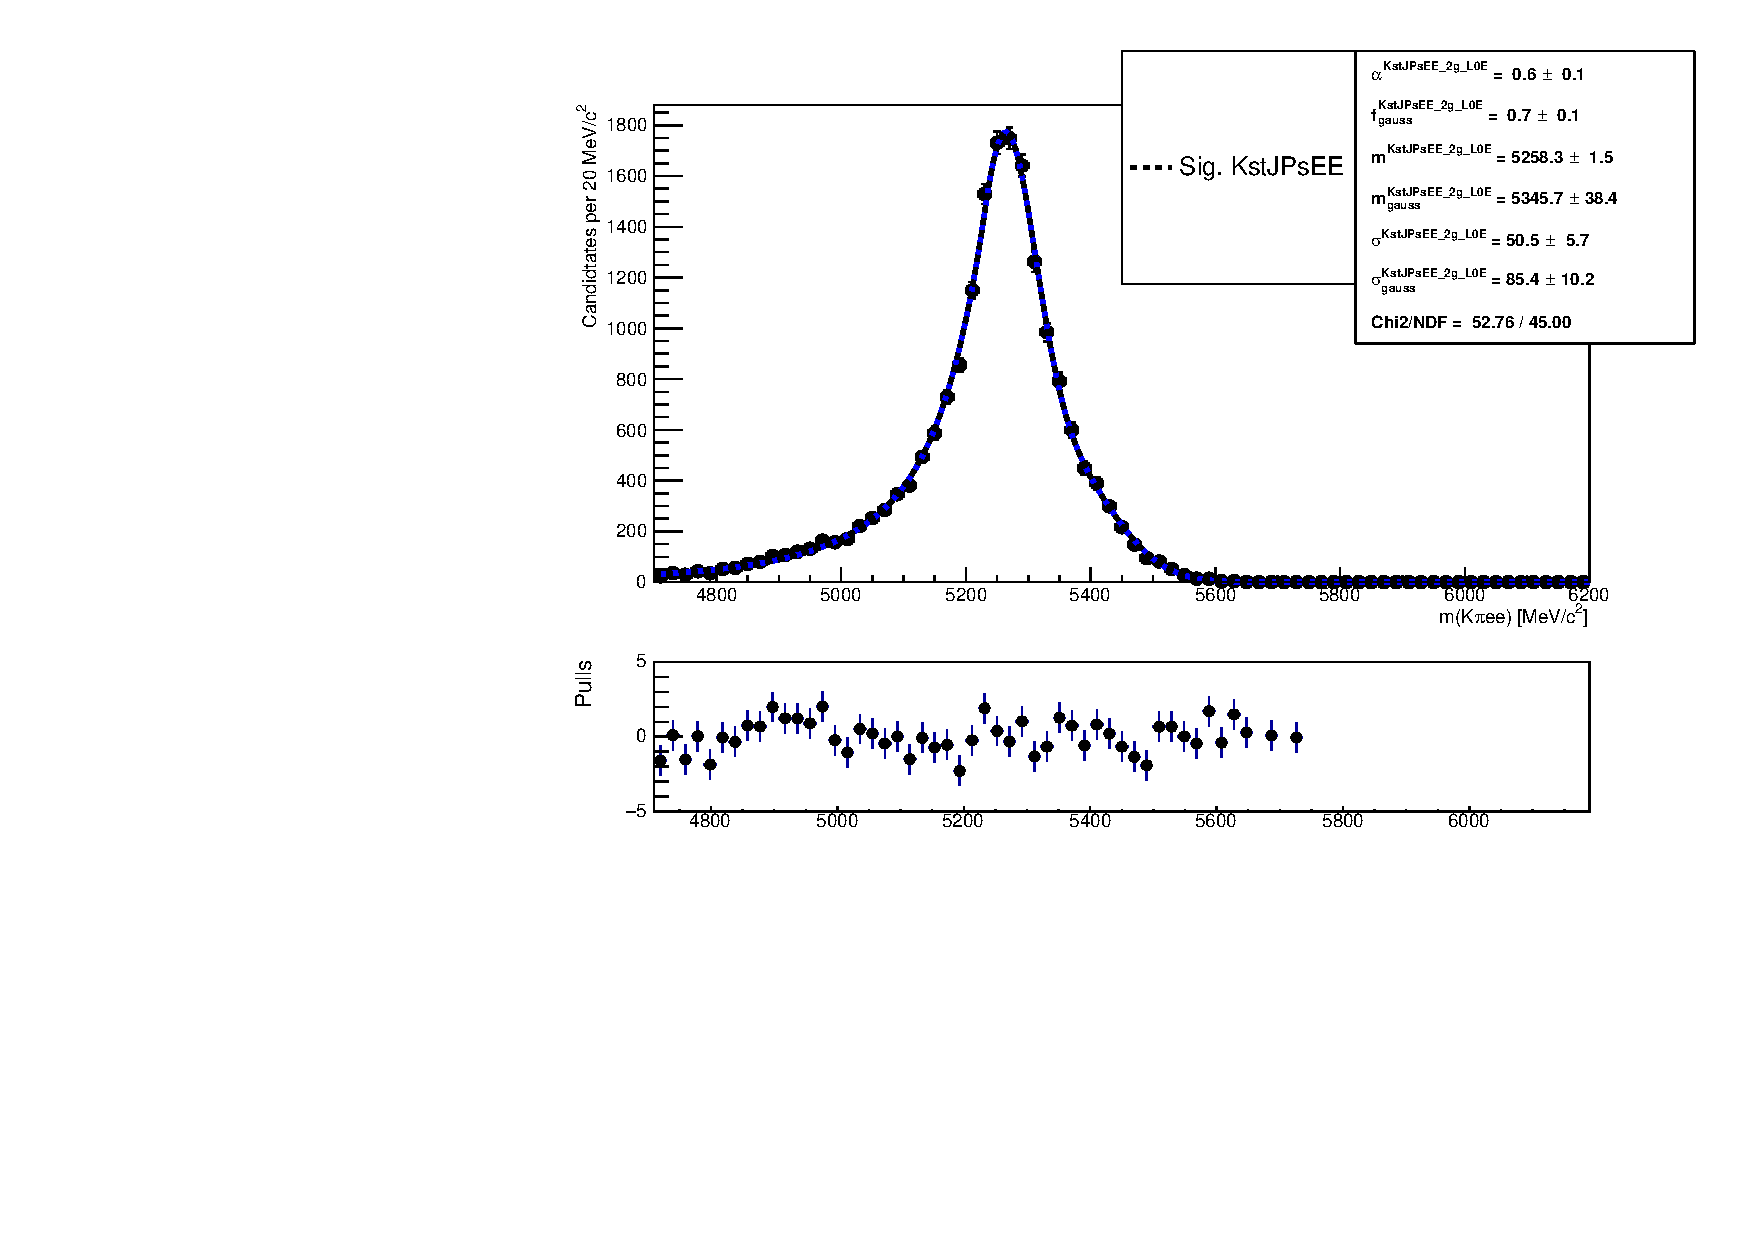
\includegraphics[width=0.6\textwidth]{RKst/figs/fit_EEs_0_EE-q2central-gmc/KstJPsEE_2g_L0E_fitAndRes.pdf}
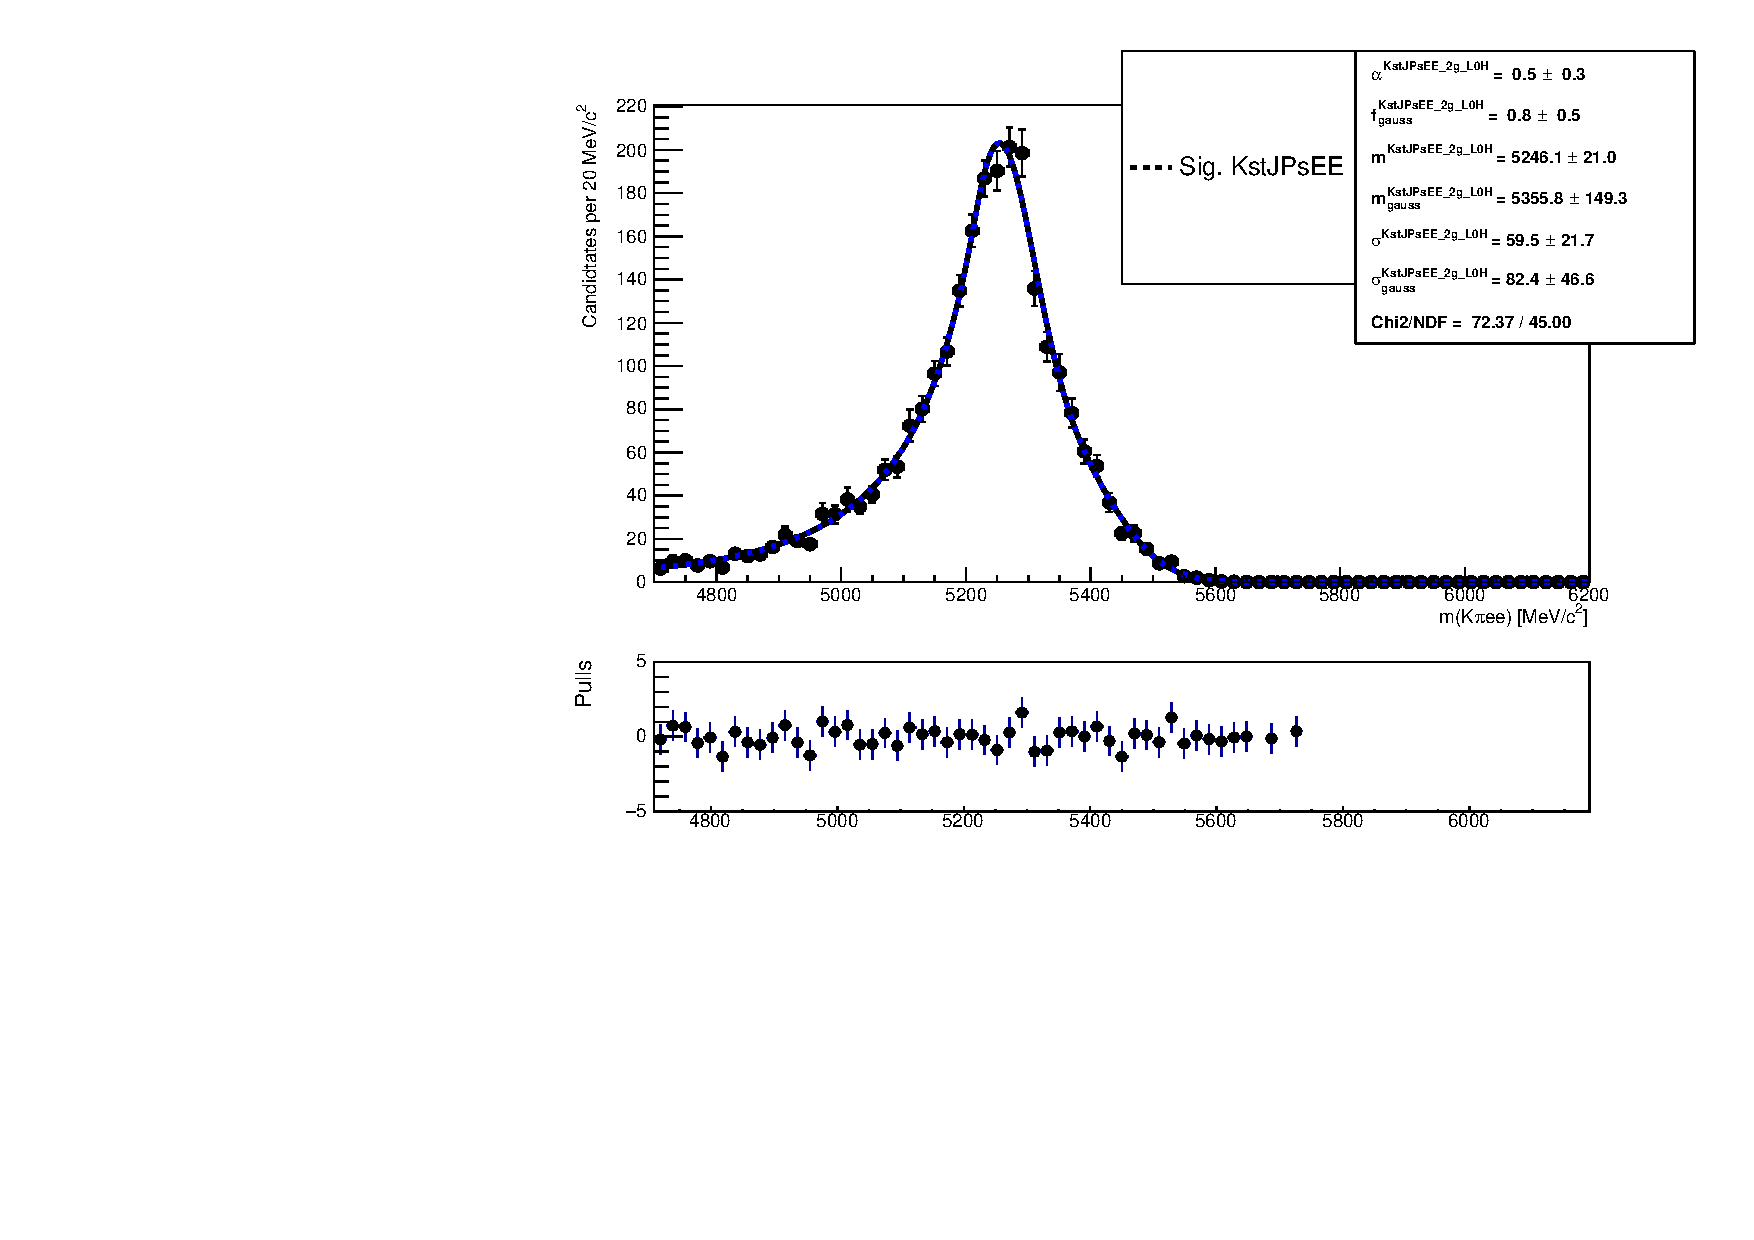
\includegraphics[width=0.6\textwidth]{RKst/figs/fit_EEs_0_EE-q2central-gmc/KstJPsEE_2g_L0H_fitAndRes.pdf}
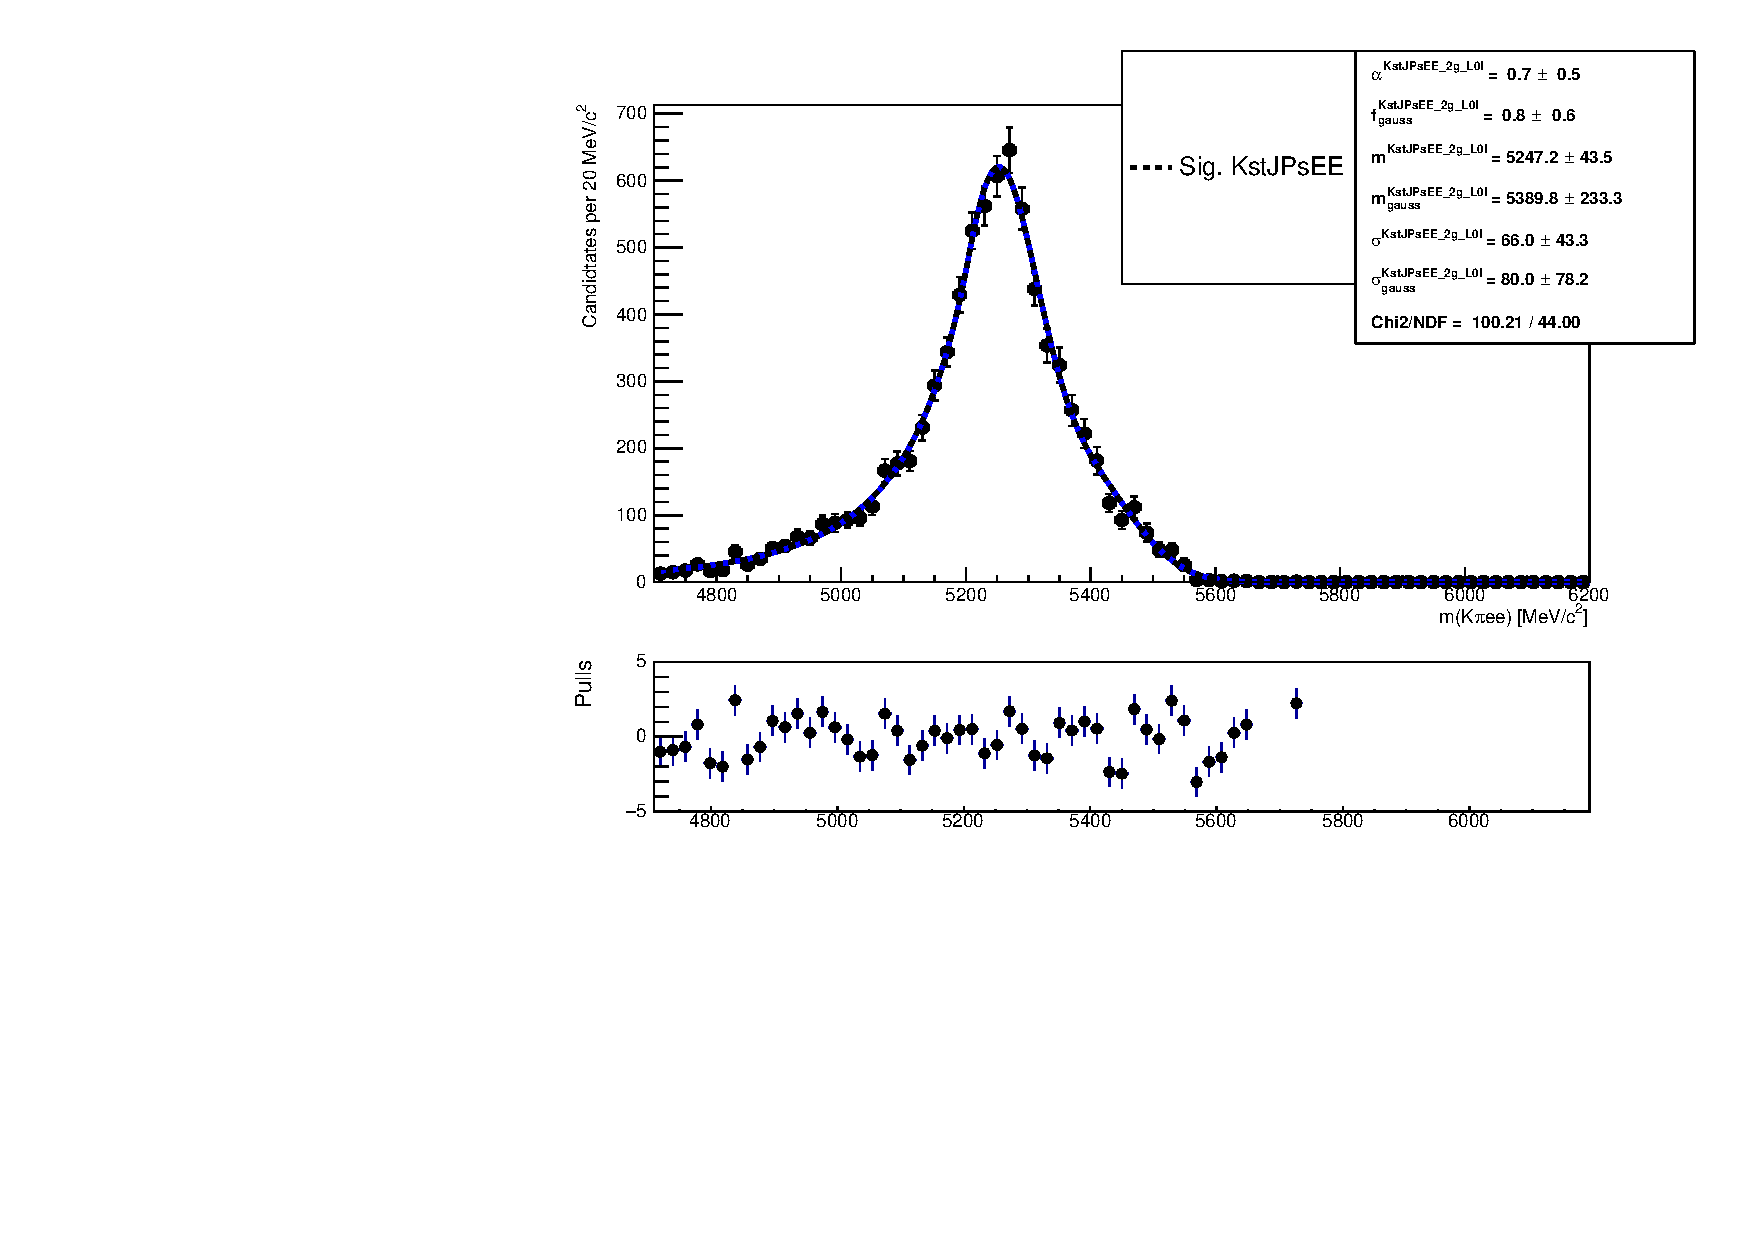
\includegraphics[width=0.6\textwidth]{RKst/figs/fit_EEs_0_EE-q2central-gmc/KstJPsEE_2g_L0I_fitAndRes.pdf}
\caption{Fitted $m(K\pi ee)$ mass spectrum of $B^0 \rightarrow K^{*0} J/\psi(J/\psi\rightarrow ee)$ simulated
events in the three trigger categories and two photons emitted. }
\label{fig:FitEE_MC_inTrigCat_Brem2}
\end{figure}